%%%%%%%%%%%%%%%%%%%%%%%%%%%%%%%%%%%%%%%%%%%%%%%%%%%%%%%%%%
%%
%% MARK: Title & Data
%%
%%%%%%%%%%%%%%%%%%%%%%%%%%%%%%%%%%%%%%%%%%%%%%%%%%%%%%%%%%

\chapter*{\S B33. Poisson Bracket in Diffeology}
\setcounter{footnote}{0}

%%%%%%%%%%%%%%%%%%%%%%%%%%%%%%%%%%%%%%%%%%%%%%%%%%%%%%%%%%
%%
%% MARK: Abstract
%%
%%%%%%%%%%%%%%%%%%%%%%%%%%%%%%%%%%%%%%%%%%%%%%%%%%%%%%%%%%

\begin{abstract}
  In this note we show how to understand the Poisson bracket in diffeology,
  working directly on the group of Hamiltonian diffeomorphisms without involving tangent spaces and Hamiltonian gradients.
  Indeed,
  as it is usually defined,
  the Poisson bracket seems to be a contravariant object and therefore not really adapted to diffeology,
  but it can be defined in a covariant way, which is more adequate to the diffeology framework.
\end{abstract}

%%%%%%%%%%%%%%%%%%%%%%%%%%%%%%%%%%%%%%%%%%%%%%%%%%%%%%%%%%
%%
%% MARK: Classical Poisson bracket
%%
%%%%%%%%%%%%%%%%%%%%%%%%%%%%%%%%%%%%%%%%%%%%%%%%%%%%%%%%%%

The question of the Poisson bracket in diffeology has been raised many times,
and recently again by Jim Stasheff in a private discussion.
This time I want to give an answer that I find satisfactory.

\section{Classical Poisson bracket}

The Poisson bracket is generally introduced in symplectic geometry as a binary operation on the space of functions.
Let $(M,\omega)$ be a symplectic manifold,
that is,
$$
  \omega \in \DForms^2(M), \quad d\omega = 0 \quad \text{and} \quad \ker(\omega) = 0.
$$
Let $x \mapsto u(x)$ be a smooth real function on $M$,
and denote its \emph{symplectic gradient} by
$$
  \grad_\omega(u) = \DForms^{-1}(du).
$$
Here $\omega$ is regarded as a linear isomorphism from $TM$ to $T^*M$,
so $\DForms^{-1}(du)$ is a tangent vector field.
The Poisson bracket is usually defined in the following way \cite{Sou70}:

\begin{Article}{The classical definition}{}
  Let $x \mapsto u(x)$ and $x \mapsto v(x)$ be two smooth real functions on $M$.%
  \footnote{They are called \emph{dynamic variables} by Souriau.}
  The \emph{Poisson bracket} of $u$ and $v$ is denoted and defined by:%
  \footnote{It is denoted by $[u,v]_P$ in \cite{Sou70}.}
  $$
    \{u,v\} = \omega(\grad_\omega(u), \grad_\omega(v)).
  $$
\end{Article}

The Poisson bracket as defined is a bilinear map
$$
  \{\cdot,\cdot\} : \Cinfty(M,\RR)^2 \to \Cinfty(M,\RR)
$$
that satisfies some classical relations, including the Jacobi identity, which we do not discuss here.

Next,
by applying the definition of the symplectic gradient,
we also have the equivalent definition:
$$
  \{u,v\} = du(\grad_\omega(v))
  \quad \text{also denoted by} \quad
  {\partial u \over \partial x}(\grad_\omega(v)).
$$

%%%%%%%%%%%%%%%%%%%%%%%%%%%%%%%%%%%%%%%%%%%%%%%%%%%%%%%%%%
%%
%% MARK: Poisson bracket in Diffeology
%%
%%%%%%%%%%%%%%%%%%%%%%%%%%%%%%%%%%%%%%%%%%%%%%%%%%%%%%%%%%

\section{Poisson bracket in diffeology}

The problem with concepts involving tangent vector fields and Lie algebras is that they have more than one interpretation in diffeology.
That is why we have to bypass, as much as possible, the introduction of tangent spaces in their generalizations in diffeology.
This works for the moment map,
relatively well,
as the many examples in \cite{PIZ10} have shown.
This is what we propose for the Poisson bracket:
a definition that covers the classical case and satisfies the constraints of a good diffeological equivalent.

Let us now return to the classical picture for a while.
Assume that the vector field
$$
  x \mapsto \grad_\omega(u)(x)
$$
is integrable.
That is,
it defines a $1$-parameter group of diffeomorphisms
$$
  t \mapsto e^{t\grad_\omega(u)}.
$$
Let us change our notation to:
$$
  Z_M : x \mapsto Z_M(x) = \grad_\omega(u)(x)
  \quad \text{and} \quad
  Z'_M : x \mapsto Z'_M(x) = \grad_\omega(u')(x).
$$
We have
$$
  \{u,u'\} = \omega_x(Z_M(x), Z'_M(x)).
$$
Assume now that $Z, Z'$ belong to the Lie algebra $\cG$ of a Lie group $G$:
$$
  Z, Z' \in \cG.
$$
The $1$-parameter groups $\{e^{t\grad_\omega(u)}\}_{t \in \RR}$ and $\{e^{t\grad_\omega(u')}\}_{t \in \RR}$ are just the actions of two $1$-parameter subgroups of $G$:
$$
  \{e^{tZ}\}_{t \in \RR}
  \quad \text{and} \quad
  \{e^{tZ'}\}_{t \in \RR}
  \quad \text{belong to} \quad
  \Hom^\infty(\RR, G),
$$
and $Z_M(x)$ and $Z'_M(x)$ are the fundamental vector fields associated with $Z$ and $Z'$ in $\cG$.
Thus,
$$
  \omega_x(Z_M(x), Z'_M(x)) = \hat x^*(\omega)(Z,Z'),
$$
where
$$
  \hat x : g \mapsto g_M(x)
$$
is the \emph{orbit map} at the point $x$ and $g_M \in \Diff(M)$ denotes the action of $G$ on $M$.
Indeed,
\begin{align*}
  \hat x^*(\omega)(Z,Z') & = \omega_x\bigl(\Der(\hat x)_{\Id_G}(Z), \Der(\hat x)_{\Id_G}(Z')\bigr) \\
  & = \omega_x\bigl(Z_M(x), Z'_M(x)\bigr),
\end{align*}
because
$$
  Z_M(x) := \left.{\partial e^{tZ}_M(x) \over \partial t}\right|_{t=0} = \Der(\hat x)_{\Id_G}(Z),
$$
where $\Id_G$ denotes the identity in $G$.

Now,

\begin{Article}{Proposition.}{}
  If the group $G$ preserves $\omega$,
  that is,
  if
  $$
    \forall g \in G, \quad g_M^*(\omega) = \omega,
  $$
  then
  $$
    \forall g \in G, \quad \Lm(g)^*(\hat x^*(\omega)) = \hat x^*(\omega),
  $$
  where $\Lm(g)$ is left multiplication in $G$.
  Thus the map $x \mapsto \hat x^*(\omega)$ defined on $M$ takes its values in the vector space of left-invariant $2$-forms on $G$.
\end{Article}

Let us denote for now
$$
  \cG_k^* = \{ \epsilon \in \DForms^k(G) \mid \forall g \in G, \ \Lm(g)^*(\epsilon) = \epsilon \}.
$$
Thus,
$$
  \{\cdot,\cdot\} = [x \mapsto \hat x^*(\omega)] \in \Cinfty(X, \cG_2^*),
$$
such that
$$
  \{\cdot,\cdot\}_x(Z,Z') = \omega_x(Z_M(x), Z'_M(x)).
$$
Returning to our symplectic gradients:
the flow $\{e^{t\grad_\omega(u)}\}_{t \in \RR}$ is called \emph{Hamiltonian} because its Hamiltonian \cite[\textsection\,9.15]{PIZ13} is $[x \mapsto u(x)]$.
Of course the group
$$
  H_\omega = \Ham(M,\omega)
$$
is not a Lie group,
but it is a diffeological group and as such obeys all diffeological constructions,
in particular the diffeological vector space of left-invariant $k$-forms on $H_\omega$ is well defined:
$$
  \cH_{\omega,k}^* = \{ \epsilon \in \DForms^k(H_\omega) \mid L(g)^*(\epsilon) = \epsilon \},
$$
for any diffeological space $X$ equipped with a closed $2$-form $\omega$.
The space $\cH_\DForms^* = \cH_{\omega,1}^*$ has already been defined as the space of \emph{momenta} of the group $H_\omega$ \cite[\textsection\,7.12]{PIZ13}.

Therefore,
we can now define the Poisson bracket in full generality:

\begin{Article}{The Poisson bracket in diffeology.}{}
  Let $(X,\omega)$ be a \uline{parasymplectic} space.
  Let $\Ham(X,\omega)$ be the group of Hamiltonian diffeomorphisms \cite[\textsection\,9.15]{PIZ13},
  and let $\cH_{\omega,2}^*$ be the diffeological vector space of left-invariant $2$-forms on $\Ham(X,\omega)$.
  We call \emph{Poisson bracket} the map
  $$
    \{\cdot, \cdot\} : x \mapsto \hat x^*(\omega),
    \qquad
    \{\cdot, \cdot\} \in \Cinfty(X, \cH_{\omega,2}^*).
  $$
  This definition coincides with the classical version when $(X,\omega)$ is a symplectic manifold.
\end{Article}

\begin{proof}
  Consider an $n$-plot $P : \U \to H_\omega$ with $P : r \mapsto g_r$,
  centered at the identity $\Id_G = P(0)$.
  Then,
  for all $x \in X$,
  for all $r \in \U$ and $\delta r, \delta'r \in \RR^n$:
  \begin{multline*}
    \{\cdot, \cdot\}_x(P)_r(\delta r, \delta'r)  = \hat x^*(\omega)(P)_r(\delta r, \delta'r)  = \omega(\hat x \circ P)_r(\delta r, \delta'r) \\
    = \omega\bigl(r \mapsto g_r(x)\bigr)_r(\delta r, \delta'r).
  \end{multline*}
  Since $\{\cdot, \cdot\}_x$ is left-invariant, it is defined by its value at the identity \cite[\textsection\,6.40, 7.18]{PIZ13}.
  Thus,
  let us compute $\{\cdot, \cdot\}_x(P)$ at $r = 0$ for two vectors $v, v' \in \RR^n$.
  \begin{multline*}
    \omega\bigl(r \mapsto g_r(x)\bigr)_0(v, v') = \omega\bigl(r \mapsto g_r(x)\bigr)_0(v, v') \\
     = \omega_{g_0(x)}\bigg( \left.{\partial g_r(x) \over \partial r}\right|_{r=0}(v),\; \left.{\partial g_r(x) \over \partial r}\right|_{r=0}(v') \bigg)
     = \omega_x\bigl(Z_M(x), Z'_M(x)\bigr),
  \end{multline*}
  where
  \begin{multline*}
    \left.{\partial g_r(x) \over \partial r}\right|_{r=0}(v) = \Der\bigl(s \mapsto g_{sv}(x)\bigr)_{s=0}(1), \quad (s \in \RR)  \\
     = \Der(\hat x)_{\Id_G}\bigg(\left.{\partial g_{sv} \over \partial s}\right|_{s=0}\bigg)
     = \Der(\hat x)_{\Id_G}(Z),
  \end{multline*}
  with
  $$
    Z = \left.{\partial g_{sv} \over \partial s}\right|_{s=0}.
  $$
  Indeed $s \mapsto g_{sv}$ is a centered path at the identity $\Id_G$,
  so its derivative defines a tangent vector $Z \in \Tgt_{\Id_G}(G)$,
  that is, an element of the Lie algebra $\cG$.
  If the action of $G$ on $M$ is Hamiltonian then $Z = \grad_\omega(u)$ and $Z' = \grad_\omega(u')$.
  Therefore:
  $$
    \omega\bigl(r \mapsto g_r(x)\bigr)_0(v, v') = \omega_x\bigl(Z_M(x), Z'_M(x)\bigr) = \{u,u'\}(x),
  $$
  which is the ordinary definition of the Poisson bracket in symplectic geometry.
\end{proof}

\begin{Article}{Remark}{}
  The Poisson bracket is not only a map from $X$ to left-invariant $2$-forms on $\Ham(X,\omega)$:
  
  (A) The Poisson bracket takes its values in the space of invariant closed $2$-forms:
  $$
    d[\{\cdot,\cdot\}(x)] = d[\hat x^*(\omega)] = \hat x^*[d\omega] = 0
    \quad \text{for all } x \in X.
  $$
  Expanded,
  this gives the \uline{Jacobi identity}.
  
  (B) Consider the special case when $\omega$ is exact and its primitive is also invariant:
  $$
    \omega = d\alpha
    \quad \text{and} \quad
    h^*(\alpha) = \alpha
    \quad \text{for all } h \in \Ham(X,\omega).
  $$
  Then,
  the Poisson bracket is related to the universal moment map $\mu_\omega$ \cite[\textsection\,9.14]{PIZ13}:
  $$
    \{\cdot,\cdot\}(x) = d[\mu_\omega(x)]
    \quad \text{for all } x \in X,
  $$
  since $\mu_\omega(x)$ is in this case simply $\hat x^*(\alpha)$.
\end{Article}

\vfill
\centerline{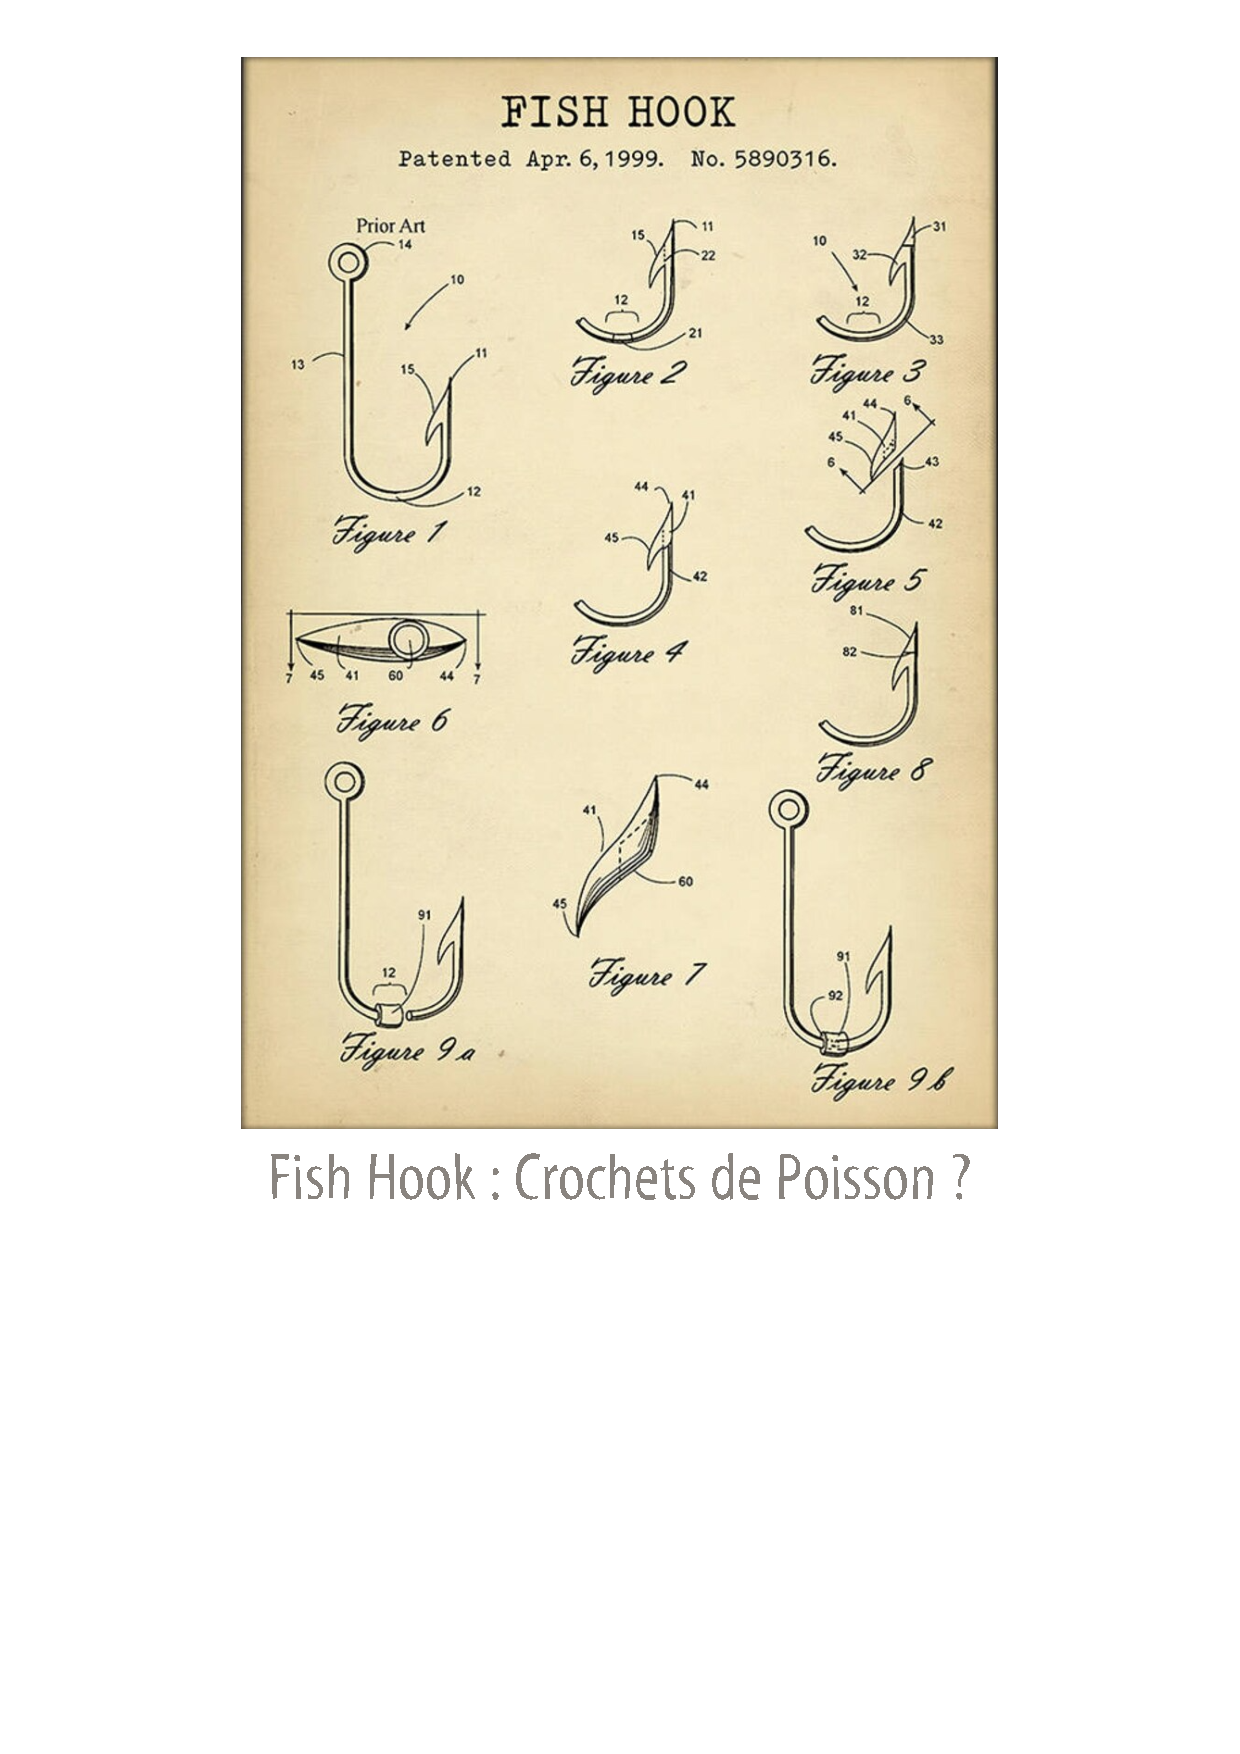
\includegraphics[width=.56\textwidth]{Figures/FishHook.pdf}}
